\documentclass[12pt]{article}
\usepackage[all, stdclass]{lix}
\usepackage{graphicx}
\usepackage{svg}
\svgsetup{
  inkscapepath=assets/,  % Path to the directory containing your SVG files
  svgpath=assets/        % Path to the directory containing your SVG files
}
\usepackage{float}
\usepackage{hyperref}
\usepackage{times}
\usepackage{amsmath}

% /main/2023-08-23-18-08-17.png - Carrier Profile
% /main/2023-08-23-18-26-49.png - Modulation
% /main/2023-08-23-18-27-00.png - Demodulation1
% /main/2023-08-23-18-27-58.png - Both Modulation and Demodulation1
% /main/2023-08-23-18-30-59.png - System

%----------EDIT COVER INFO HERE -----------------%

\def \LOGOPATH {assets/birzeit-logo.png}
\def \DEPARTEMENT {Department of Electrical \& Computer Engineering}
\def \COURSENUM {ENEE4113}
\def \COURSENAME {Communications Laboratory}
\def \REPORTTITLE {Ampiltude Shift Keying (ASK)}
\def \STUDENTNAME {Mohammad Abu-Shelbaia}
\def \STUDENTID {1200198}
\def \INSTRUCTOR {Dr. Ibrahim Nemer}
\def \ASSISTANT {Eng. Mohammad Al-Battat}
\def \REPORTNUM {10}

\begin{document}
\pagenumbering{Roman}

\begin{titlepage}
    \vfill
    \begin{center}
        \includegraphics[width=0.7\textwidth]{\LOGOPATH} \\
        \hfill \\
        \Large{\DEPARTEMENT} \\
        \Large{\COURSENUM\;-\;\COURSENAME} \\
        \vfill
        \textbf{\LARGE{Experiment \#\REPORTNUM}} \\
        \textbf{\LARGE{\REPORTTITLE}}
    \end{center}
    \vfill
    \begin{flushleft}
        \Large{\textbf{Prepared by:}\\ \STUDENTNAME\quad\STUDENTID} \\

        \Large{\textbf{Instructor:} \INSTRUCTOR} \\
        \Large{\textbf{Assistant:} \ASSISTANT} \\
        \Large{\textbf{Section:} 4}\\
        \LARGE{\textbf{ }}\\
        \LARGE{\textbf{ }}\\
        \LARGE{\textbf{ }}\\
        \Large{\textbf{Date:} \today}\\
    \end{flushleft}
    \vfill
\end{titlepage}


%--------------- TABLES --------------------------------%
\tableofcontents
\clearpage
\setlength{\parskip}{\baselineskip}%
\listoffigures
\clearpage
% \listoftables
% \clearpage
\pagenumbering{arabic}
%-------------- CONTENT ---------------------%
\h{Simulation and Data Analysis}
\begin{figure}[H]
    \centering
    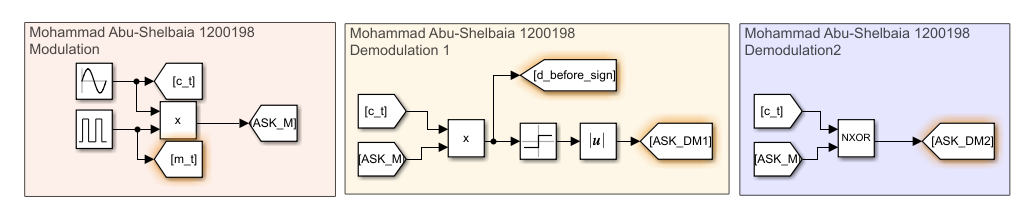
\includegraphics[width=1\textwidth]{assets/main/2023-08-23-18-30-59.png}
    \caption{Modulation/Demodulation Simulink Block Diagram}
\end{figure}
The above system is simulated using MATLAB Simulink for different messages modulated over a carrier signal with a frequency of 20KHz.
\begin{equation}
    c(t) = \cos(2\pi(20k)t)
\end{equation}
\hh{Input Signals}
\begin{figure}[H]
    \centering
    \resizebox{0.49\textwidth}{0.23\textwidth}{
    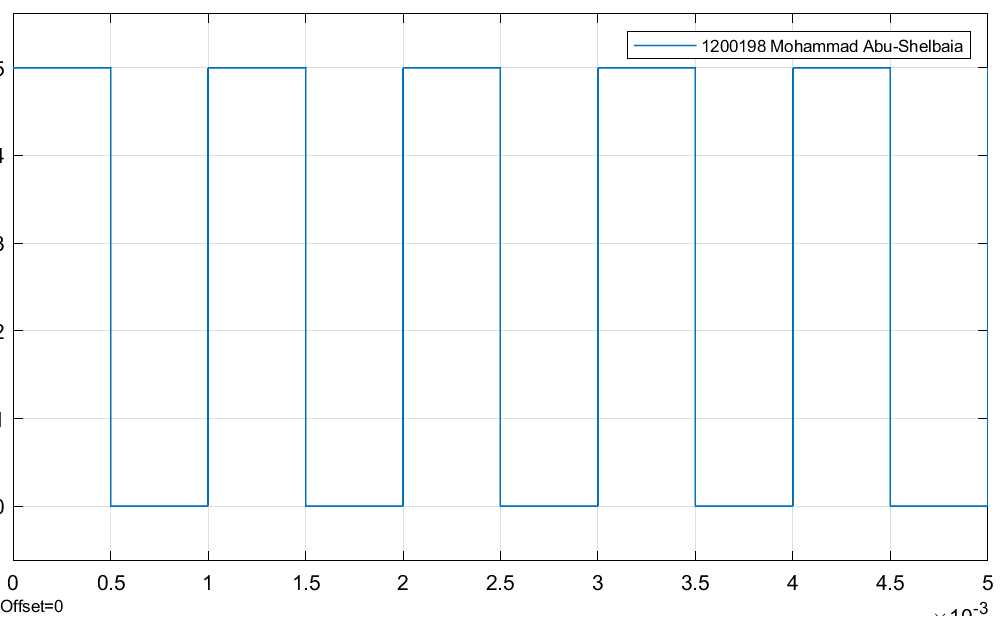
\includegraphics[width=\textwidth]{assets/main/2023-08-23-18-56-06.png}
    }
    \resizebox{0.49\textwidth}{0.23\textwidth}{
        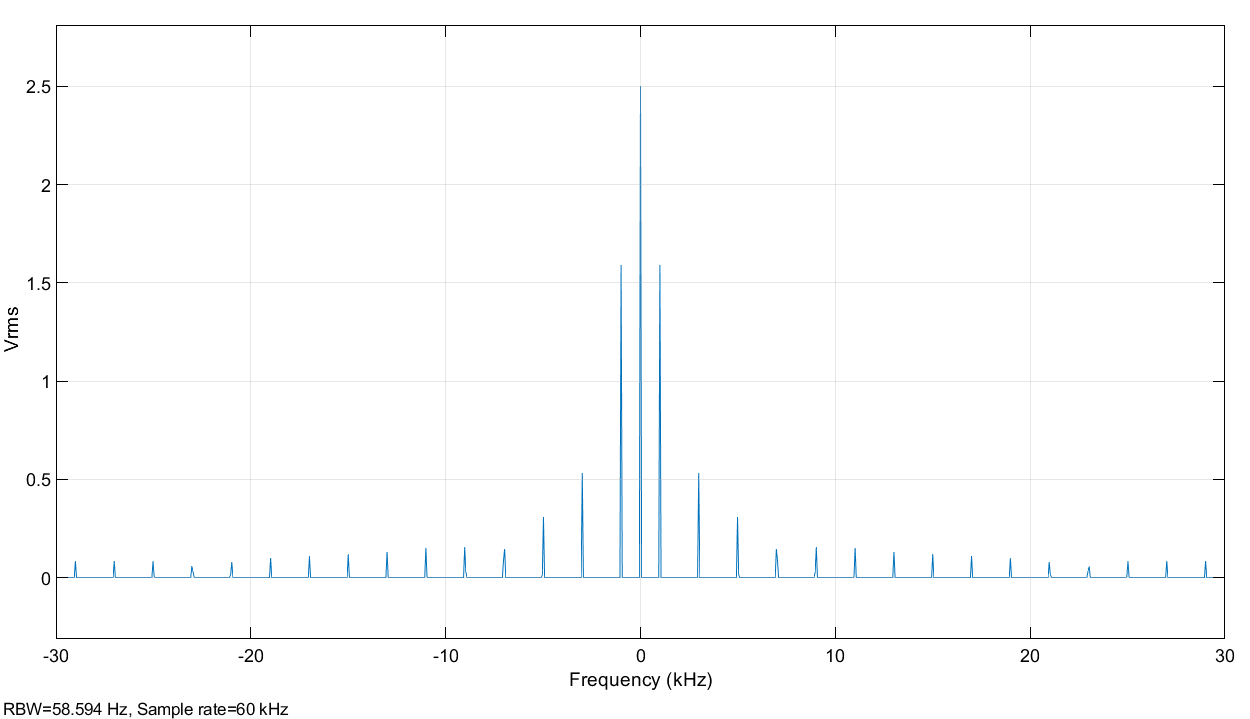
\includegraphics[width=\textwidth]{assets/main/2023-08-23-19-13-47.png}
    }
    \caption{Message Signal}
\end{figure}
\begin{figure}[H]
    \centering
    \resizebox{0.49\textwidth}{0.23\textwidth}{
    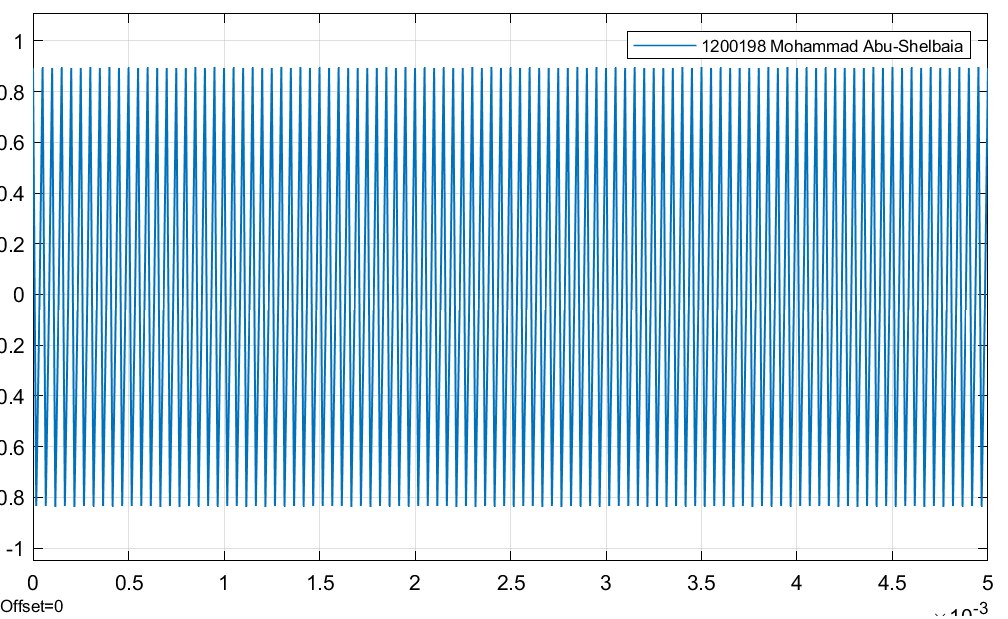
\includegraphics[width=\textwidth]{assets/main/2023-08-23-18-54-41.png}
    }
    \resizebox{0.49\textwidth}{0.23\textwidth}{
        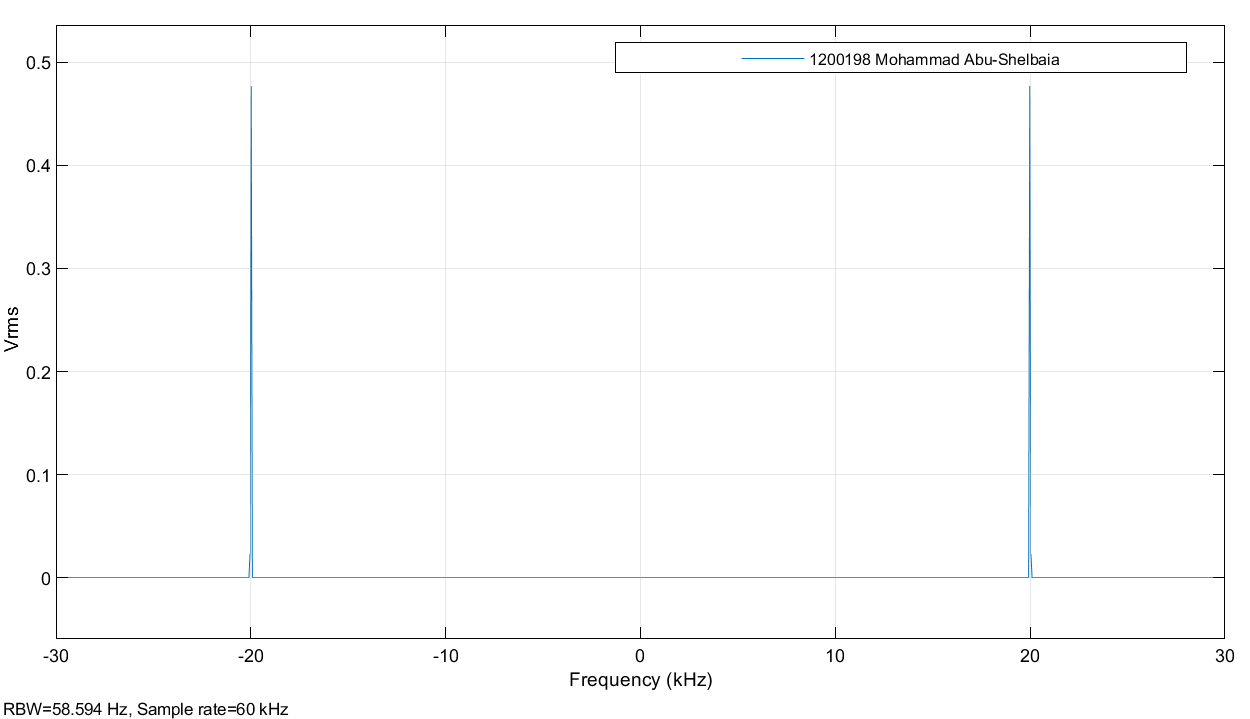
\includegraphics[width=\textwidth]{assets/main/main/2023-08-23-18-51-29.png.png}
    }
    \caption{Carrier Signal}
\end{figure}
\hh{Charchterstics of the ASK Modulated Signal}
To observer the characteristics of the ASK modulated signal, we are going to modulate a signal with low-voltage (0V) and high-voltage (2.5V) over the same carrier.

\begin{figure}[H]
    \centering
    \resizebox{0.49\textwidth}{0.25\textwidth}{
    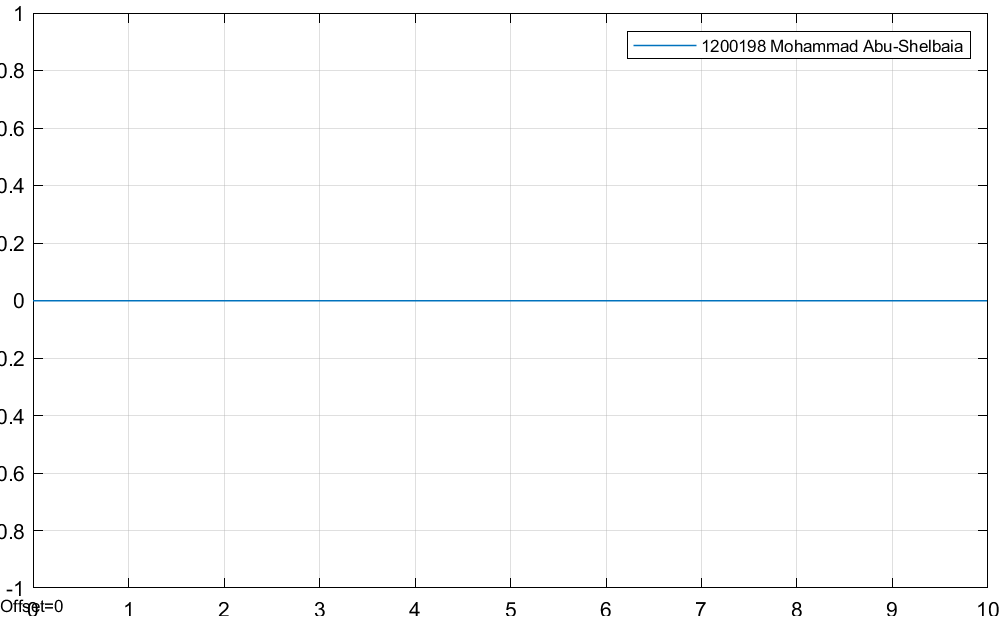
\includegraphics[width=\textwidth]{assets/main/2023-08-23-19-23-47.png}
    }
    \resizebox{0.49\textwidth}{0.25\textwidth}{
        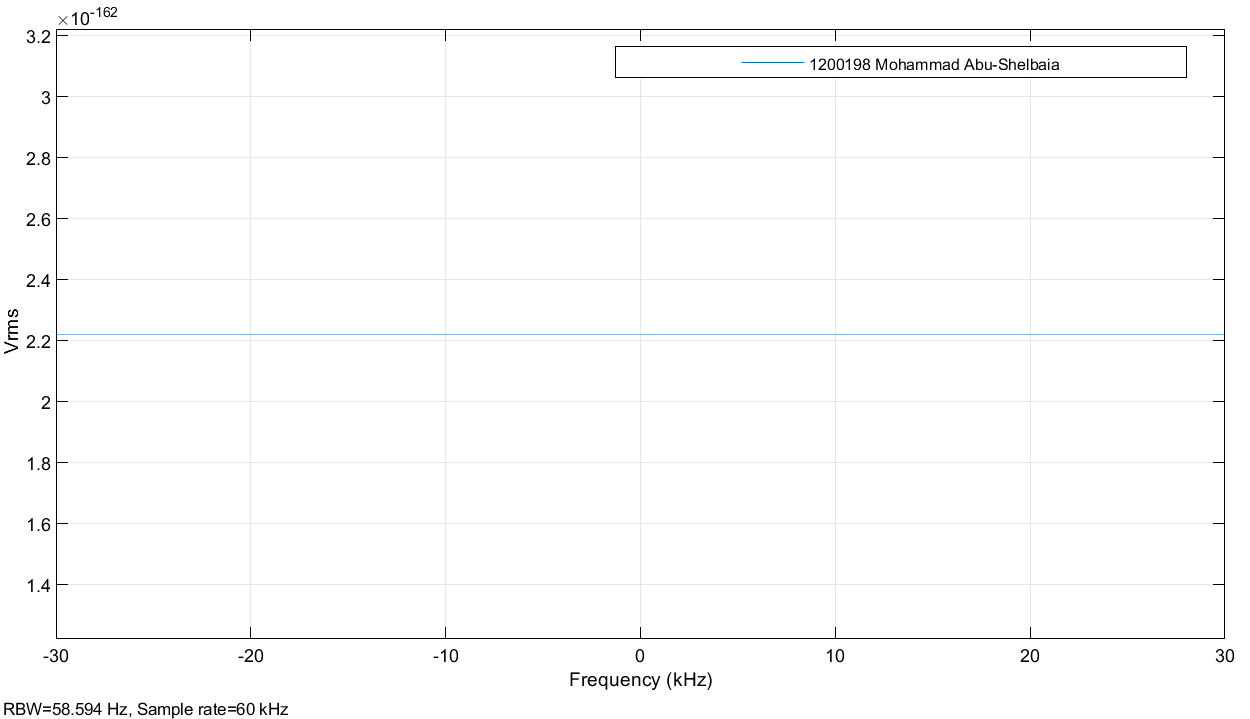
\includegraphics[width=\textwidth]{assets/main/2023-08-23-19-24-12.png}
    }
    \caption{Low voltage Modulating Signal (0V)}
\end{figure}
\begin{figure}[H]
    \centering
    \resizebox{0.49\textwidth}{0.25\textwidth}{
    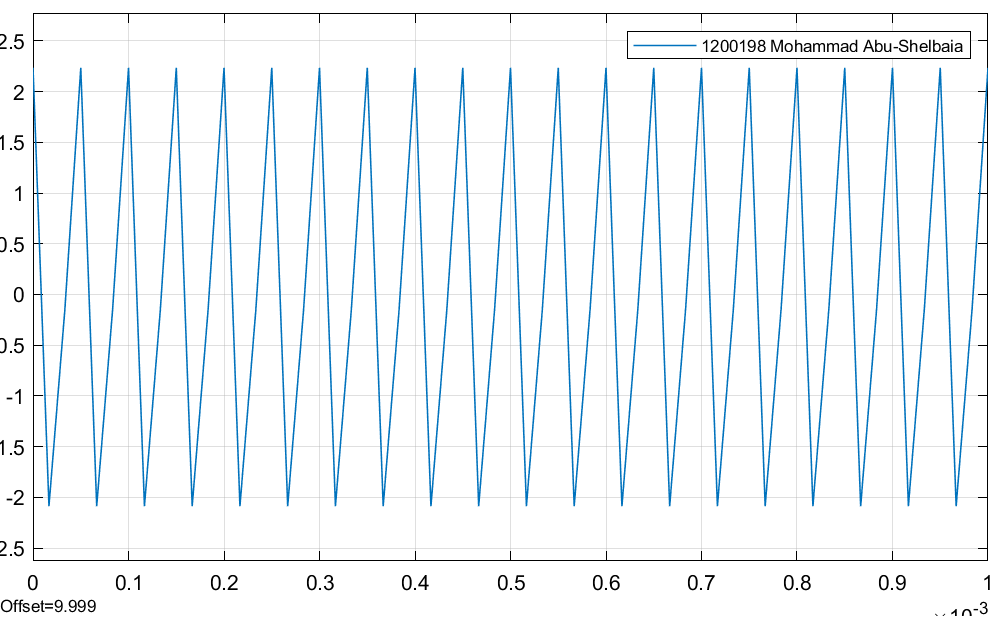
\includegraphics[width=\textwidth]{assets/main/2023-08-23-19-28-33.png}
    }
    \resizebox{0.49\textwidth}{0.25\textwidth}{
        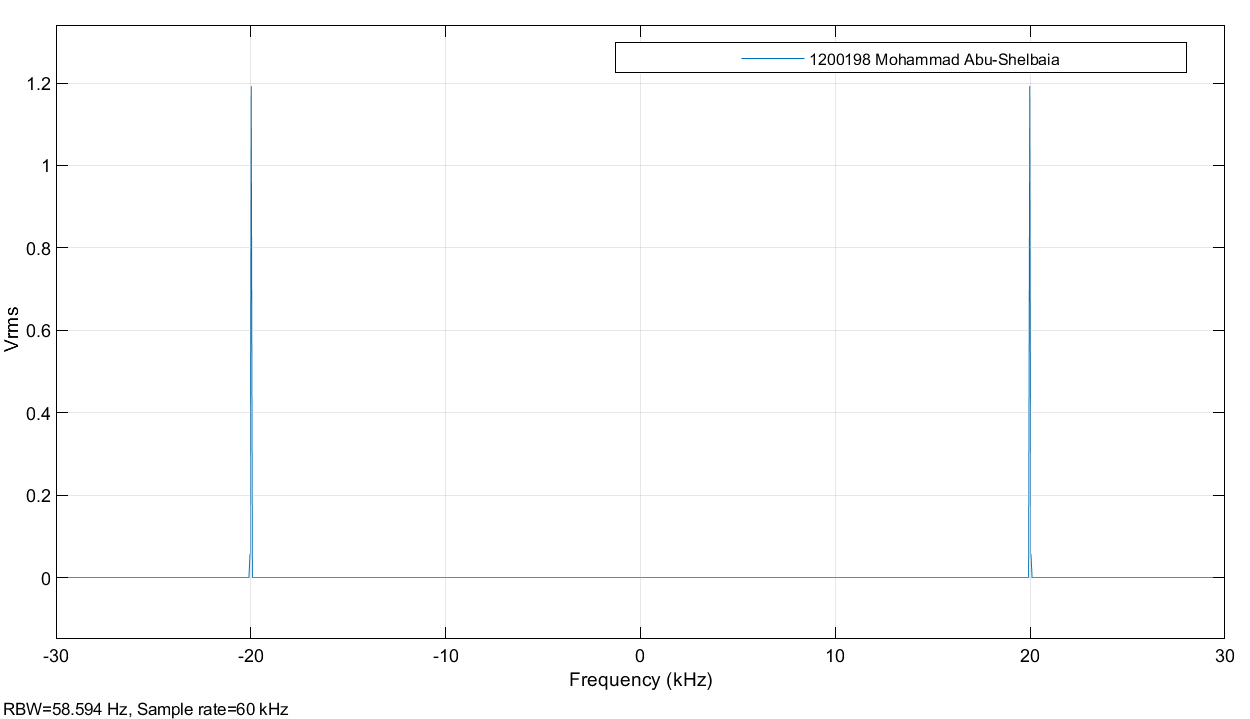
\includegraphics[width=\textwidth]{assets//main/2023-08-23-19-28-50.png}
    }
    \caption{High voltage Modulating Signal (2.5V)}

\end{figure}
We observed that whenever we send a high voltage signal, the carrier singal is transmitted as it is, and whenever we send a low voltage signal nothing is transmitted (zero signal).

\hh{Modulation and Demodulation}
\hhh{Refrence Modulating Signal}
This is our refrence modulating signal, which is a pulse-train with a frequency of 1KHz, duty cycle of 50\%, and an amplitude of 5V.
\begin{figure}[H]
    \centering
    \resizebox{0.49\textwidth}{0.25\textwidth}{
    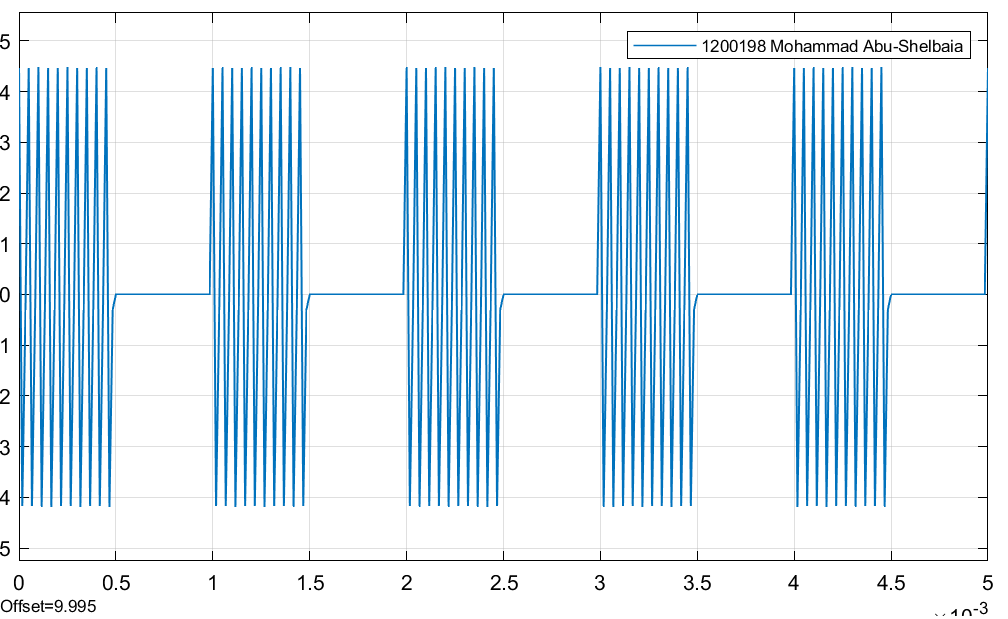
\includegraphics[width=\textwidth]{assets/main/2023-08-23-19-39-25.png}
    }
    \resizebox{0.49\textwidth}{0.25\textwidth}{
        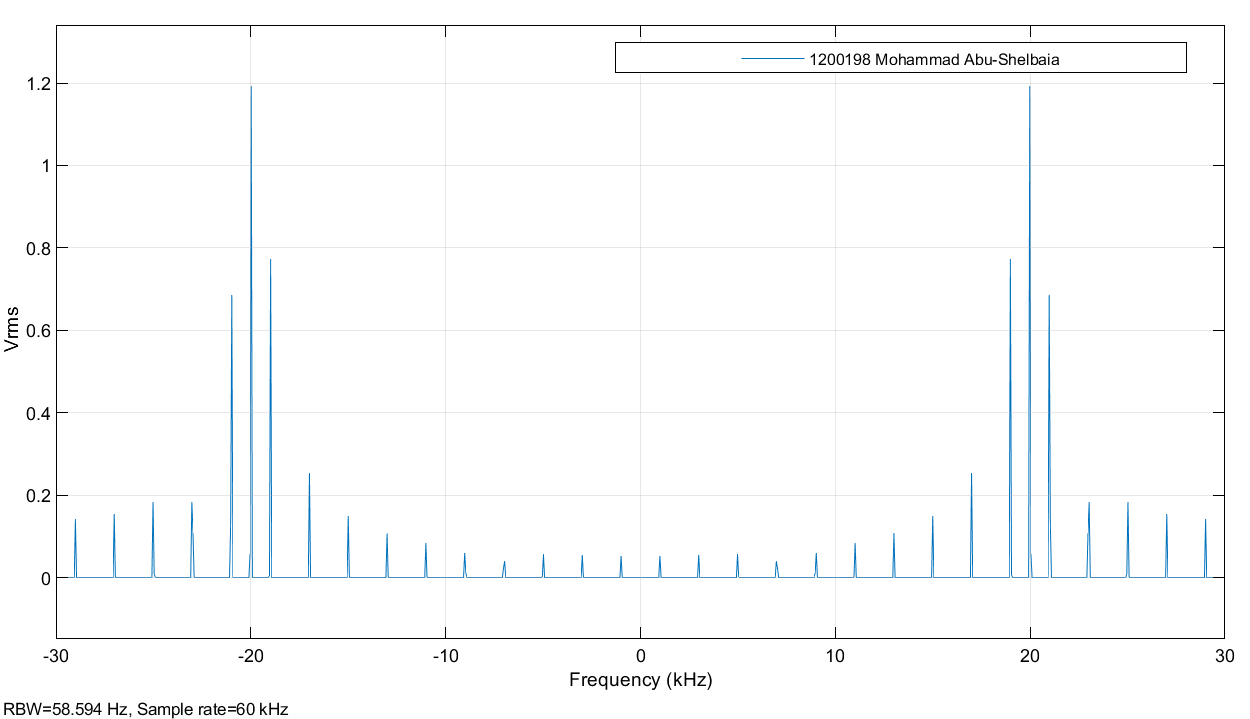
\includegraphics[width=\textwidth]{assets/main/2023-08-23-19-39-38.png}
    }
    \caption{Modulated Singal}
\end{figure}
We can see that the modulated signal is a cosine wave when the message signal is high, and zero when the message signal is low.
\begin{figure}[H]
    \centering
    \resizebox{0.49\textwidth}{0.25\textwidth}{
    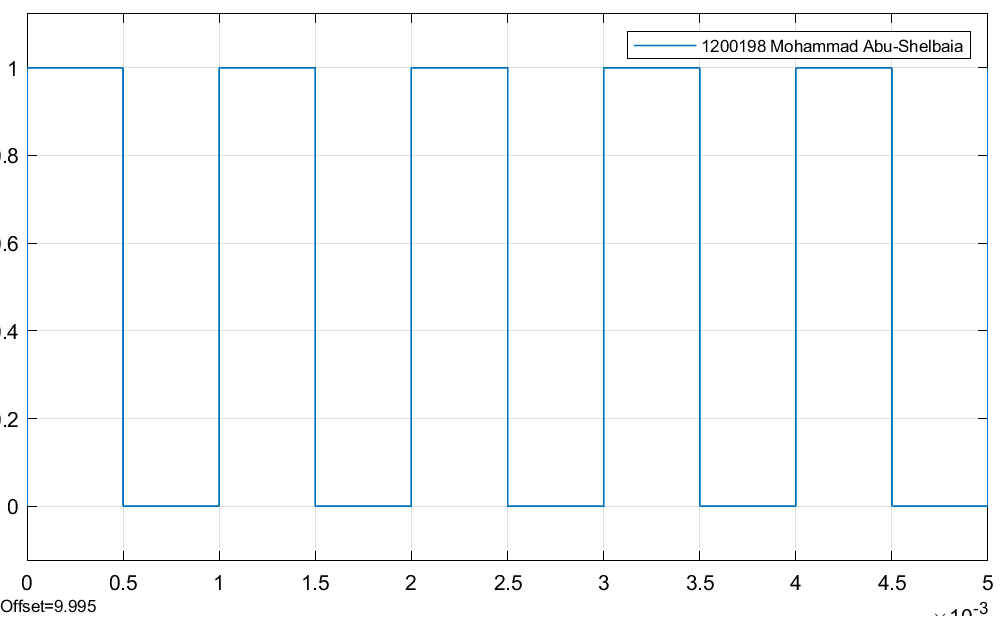
\includegraphics[width=\textwidth]{assets/main/2023-08-23-19-43-20.png}
    }
    \resizebox{0.49\textwidth}{0.25\textwidth}{
        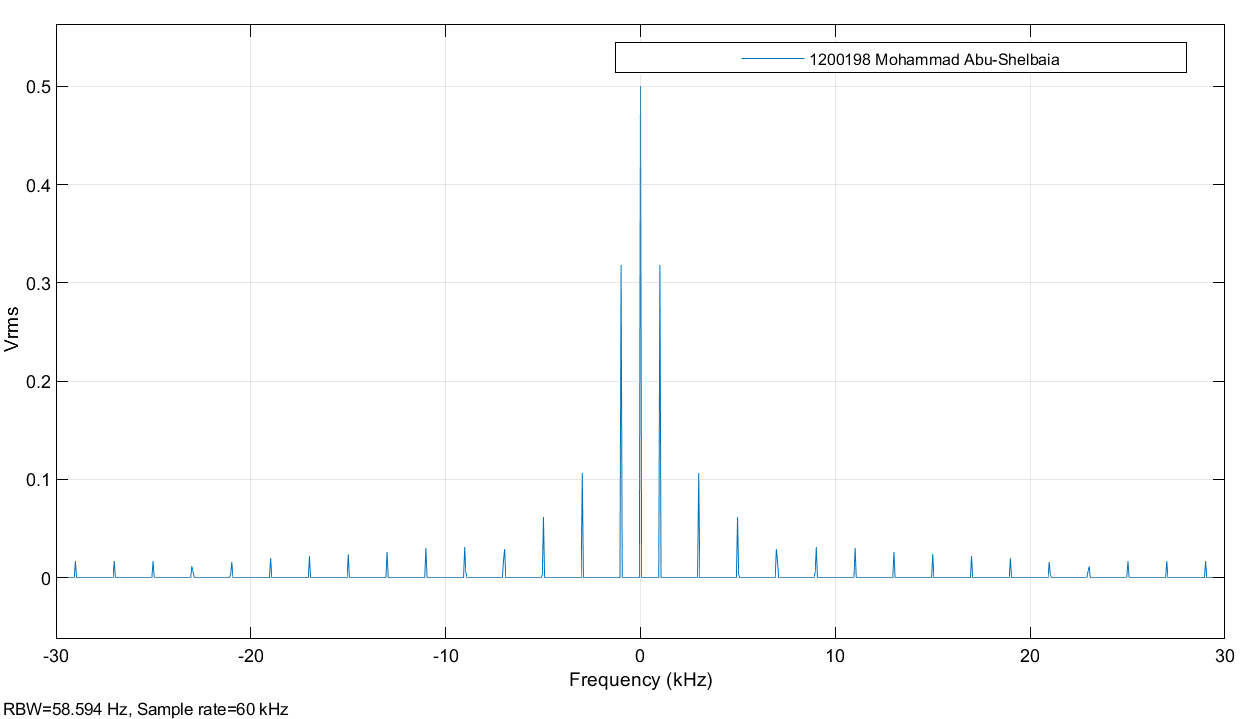
\includegraphics[width=\textwidth]{assets/main/2023-08-23-19-43-35.png}
    }
    \caption{Demodulaed Singal Method 1}
\end{figure}
\begin{figure}[H]
    \centering
    \resizebox{0.49\textwidth}{0.25\textwidth}{
        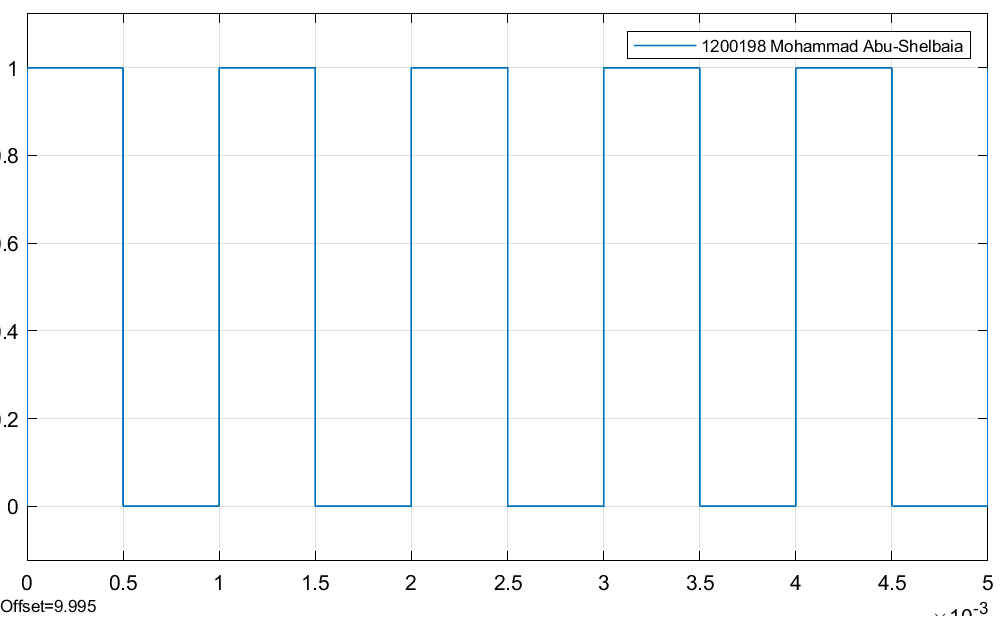
\includegraphics[width=\textwidth]{assets//main/2023-08-23-19-47-11.png}
        }
        \resizebox{0.49\textwidth}{0.25\textwidth}{
            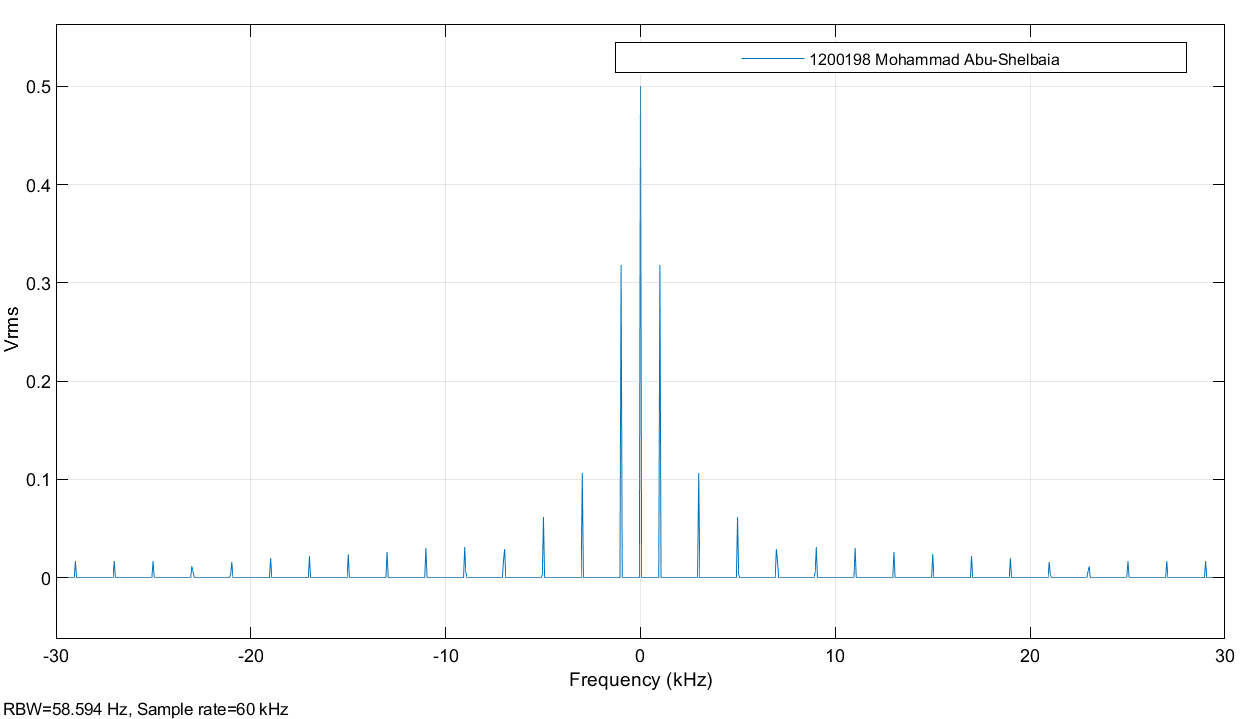
\includegraphics[width=\textwidth]{assets/main/2023-08-23-19-45-03.png}
    }
    \caption{Demodulated Singal Method 2}
\end{figure}
We can see that we have successfully demodulated the signal using both methods, the high portion of the message singal is recoverd as 1, and the low portion is recovered as 0.
\hhh{1.5V Modulating Signal}
\begin{figure}[H]
    \centering
    \resizebox{0.49\textwidth}{0.25\textwidth}{
    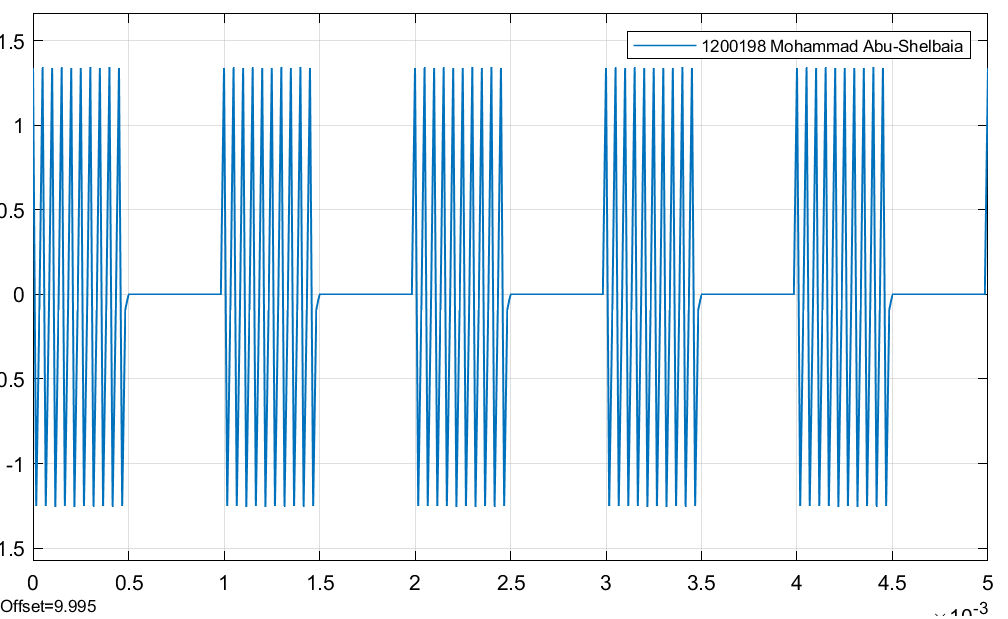
\includegraphics[width=\textwidth]{assets/main/2023-08-23-19-51-55.png}
    }
    \resizebox{0.49\textwidth}{0.25\textwidth}{
        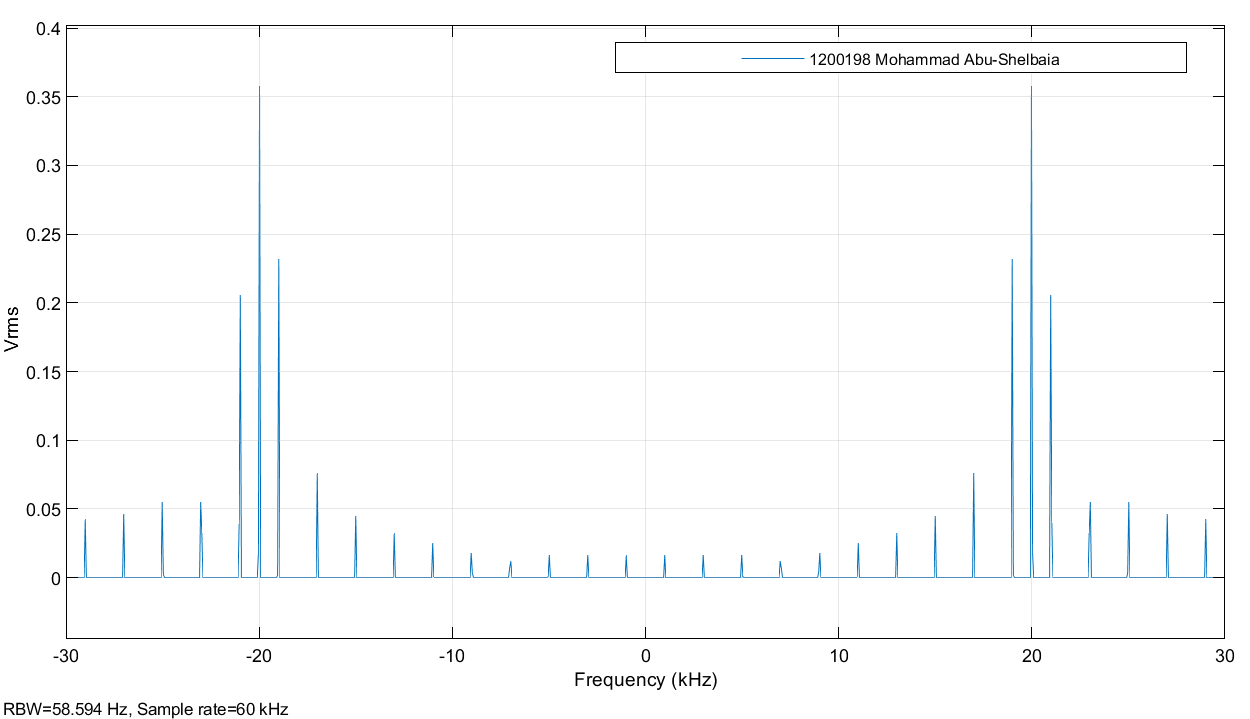
\includegraphics[width=\textwidth]{assets/main/2023-08-23-19-51-44.png}
    }
    \caption{Modulated Singal (1.5V)}
\end{figure}

We can see that the modulated signal amplitude is lower, but the same characteristics are still there.
\begin{figure}[H]
    \centering
    \resizebox{0.49\textwidth}{0.25\textwidth}{
    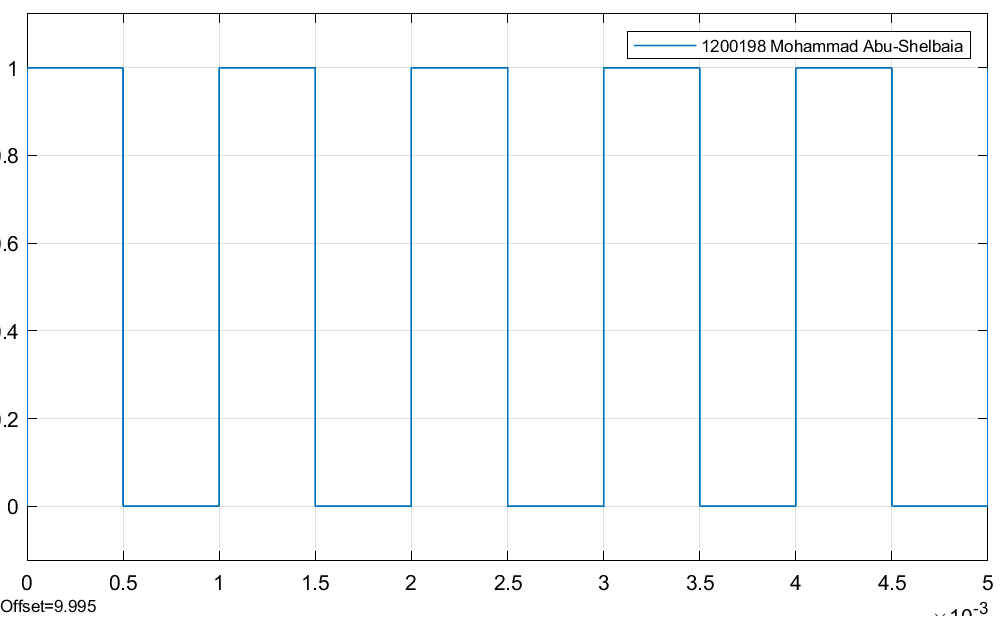
\includegraphics[width=\textwidth]{assets/main/2023-08-23-19-54-01.png}
    }
    \resizebox{0.49\textwidth}{0.25\textwidth}{
        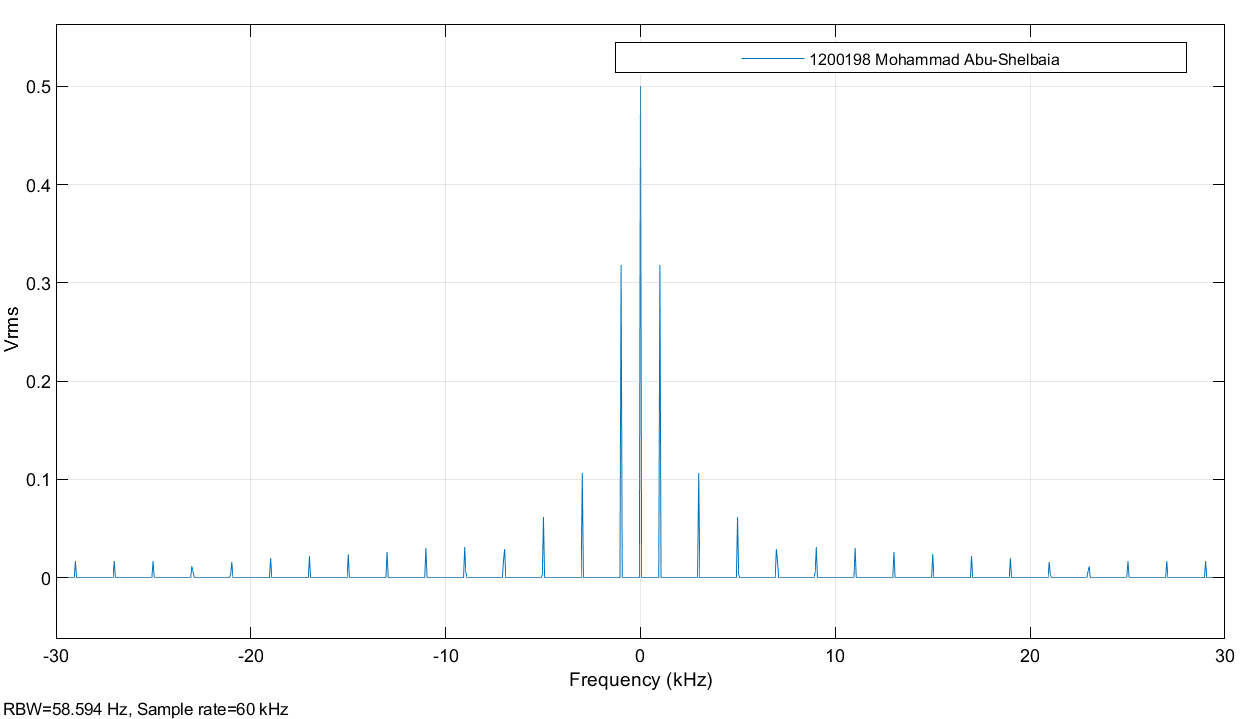
\includegraphics[width=\textwidth]{assets//main/2023-08-23-19-54-17.png}
    }
    \caption{Demodulated Singal Method 1 (1.5V)}
\end{figure}
\begin{figure}[H]
    \centering
    \resizebox{0.49\textwidth}{0.25\textwidth}{
    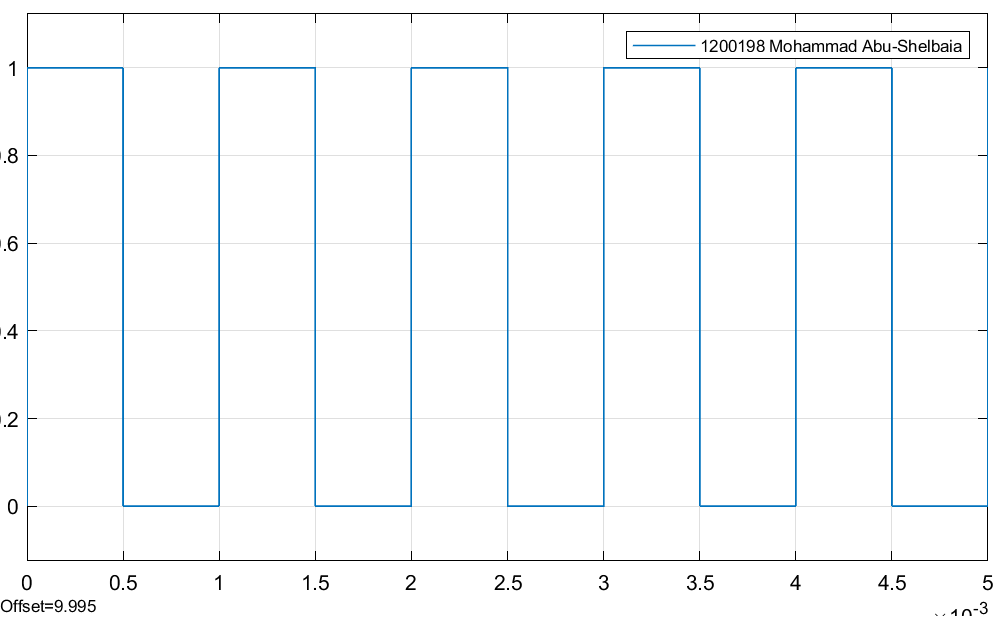
\includegraphics[width=\textwidth]{assets/main/2023-08-23-19-54-42.png}
    }
    \resizebox{0.49\textwidth}{0.25\textwidth}{
        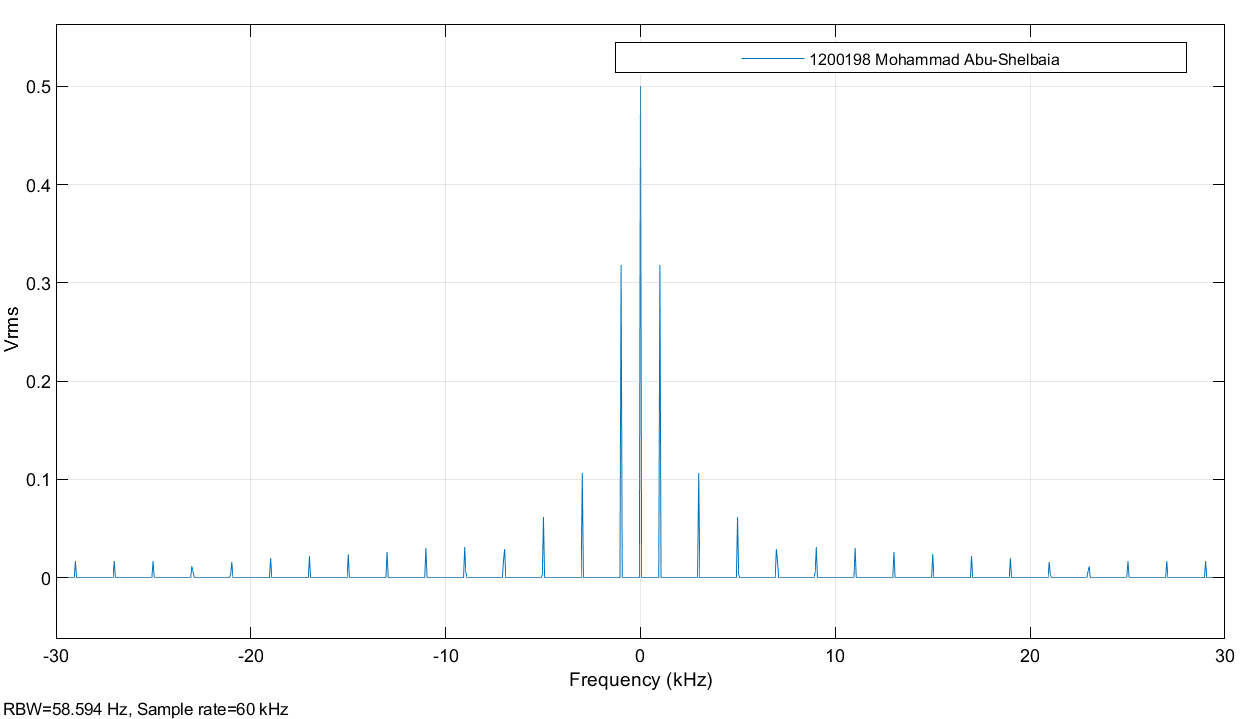
\includegraphics[width=\textwidth]{assets/main/2023-08-23-19-55-03.png}
    }
    \caption{Demodulated Singal Method 2 (1.5V)}
\end{figure}
We can see the same results as before, the high portion of the message singal is recoverd as one, and the low portion is recovered as zero.
\hhh{500Hz Modulating Signal}
\begin{figure}[H]
    \centering
    \resizebox{0.49\textwidth}{0.25\textwidth}{
    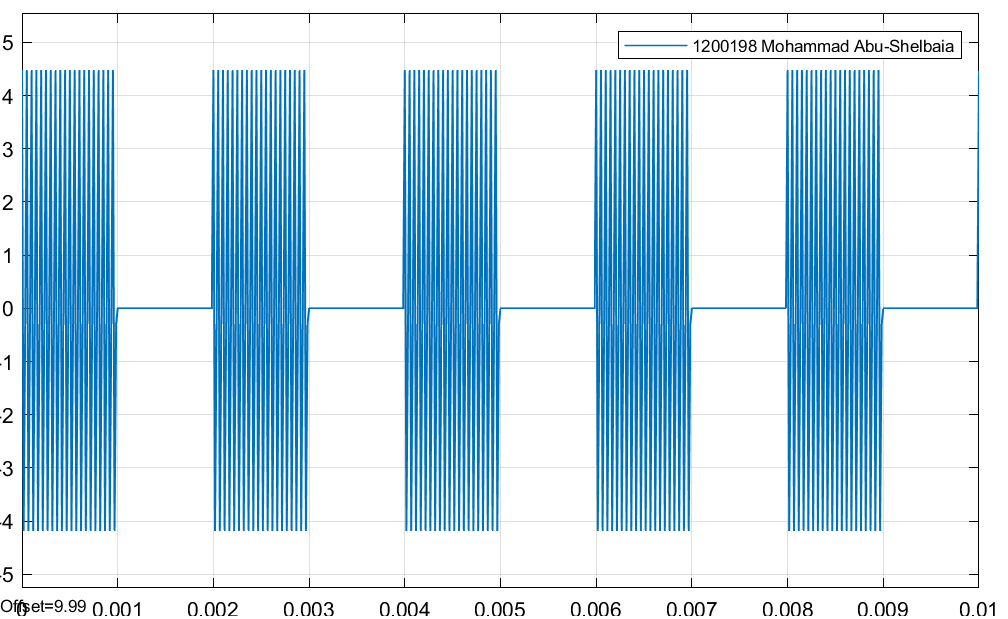
\includegraphics[width=\textwidth]{assets/main/2023-08-23-20-04-04.png}
    }
    \resizebox{0.49\textwidth}{0.25\textwidth}{
        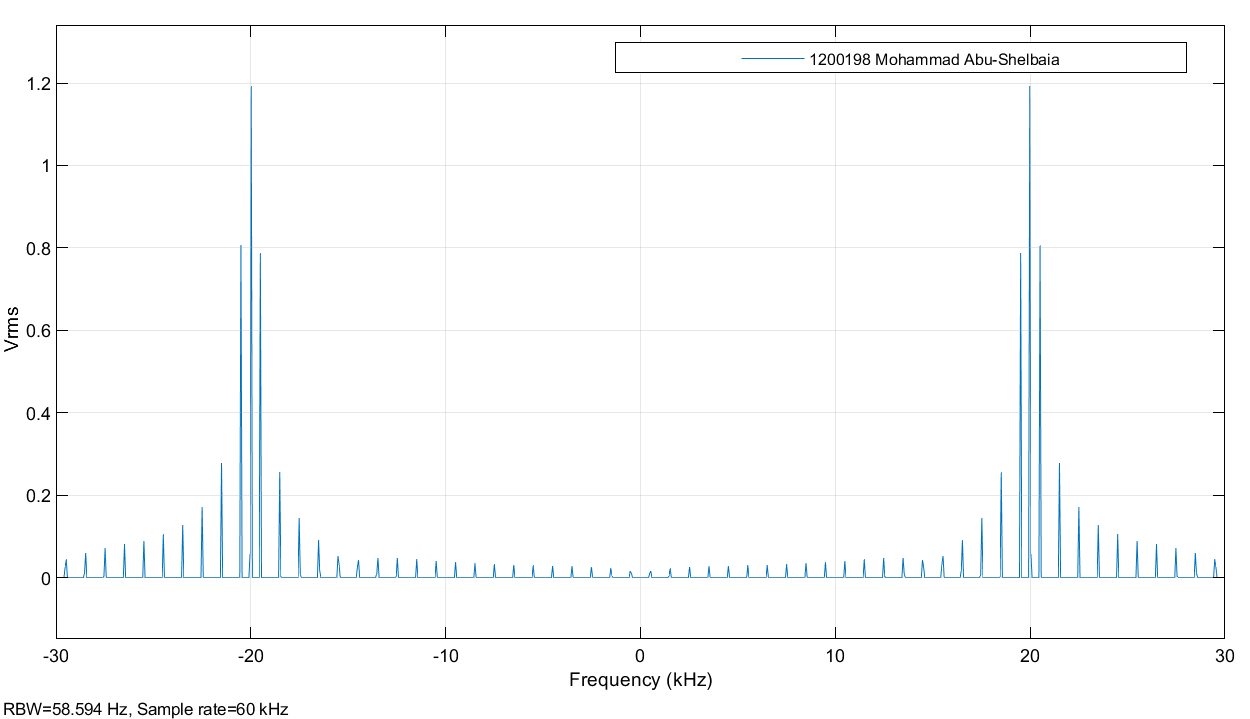
\includegraphics[width=\textwidth]{assets/main/2023-08-23-20-04-20.png}
    }
    \caption{Modulated Singal (500Hz)}
\end{figure}
We can see that the modulated signal is just more dense, but the same characteristics are still there.
\begin{figure}[H]
    \centering
    \resizebox{0.49\textwidth}{0.25\textwidth}{
    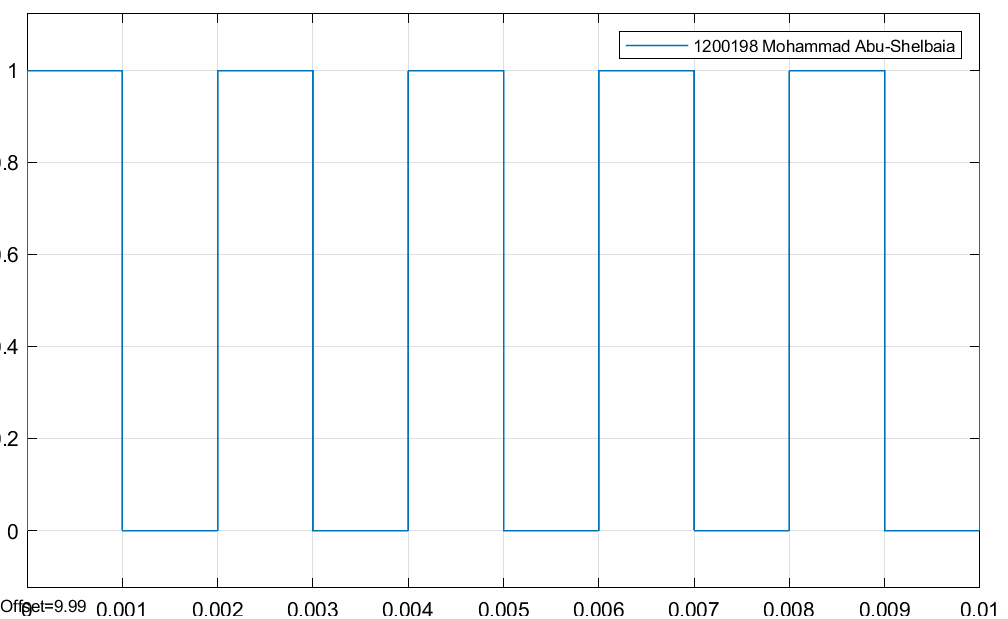
\includegraphics[width=\textwidth]{assets/main/2023-08-23-20-08-22.png}
    }
    \resizebox{0.49\textwidth}{0.25\textwidth}{
        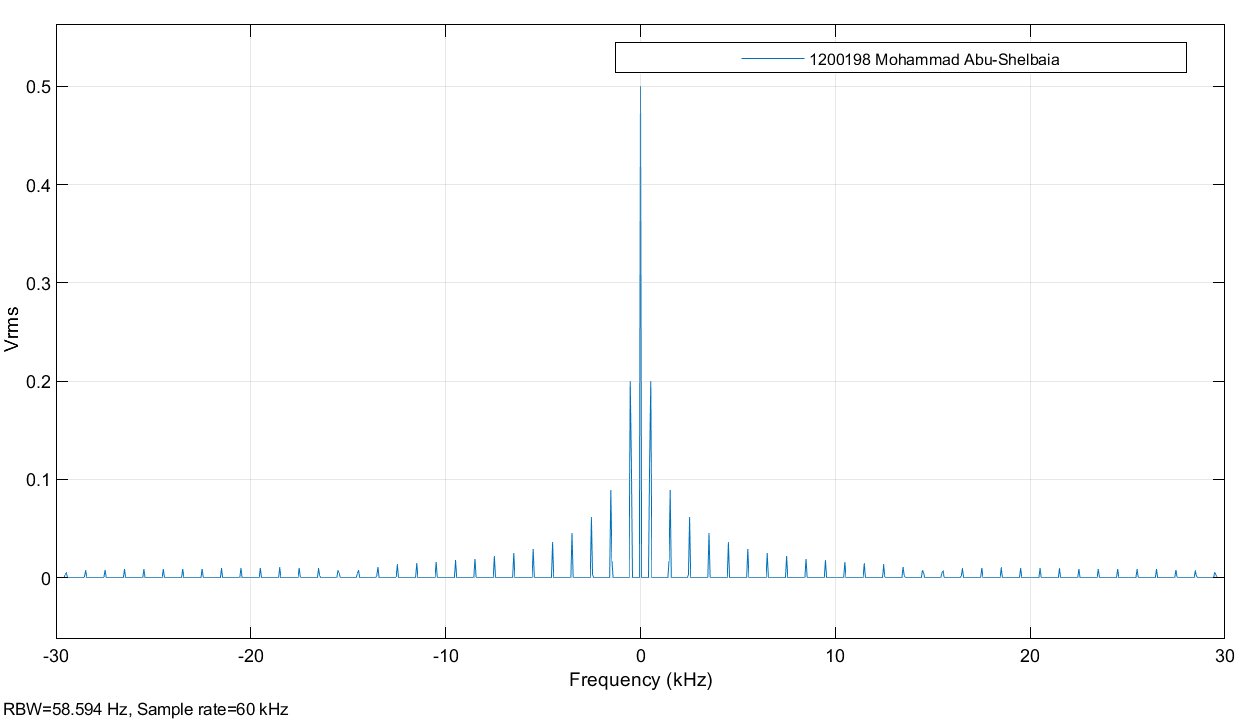
\includegraphics[width=\textwidth]{assets/main/2023-08-23-20-09-05.png}
    }
    \caption{Demodulated Singal Method 1 (500Hz)}
\end{figure}
\begin{figure}[H]
    \centering
    \resizebox{0.49\textwidth}{0.25\textwidth}{
    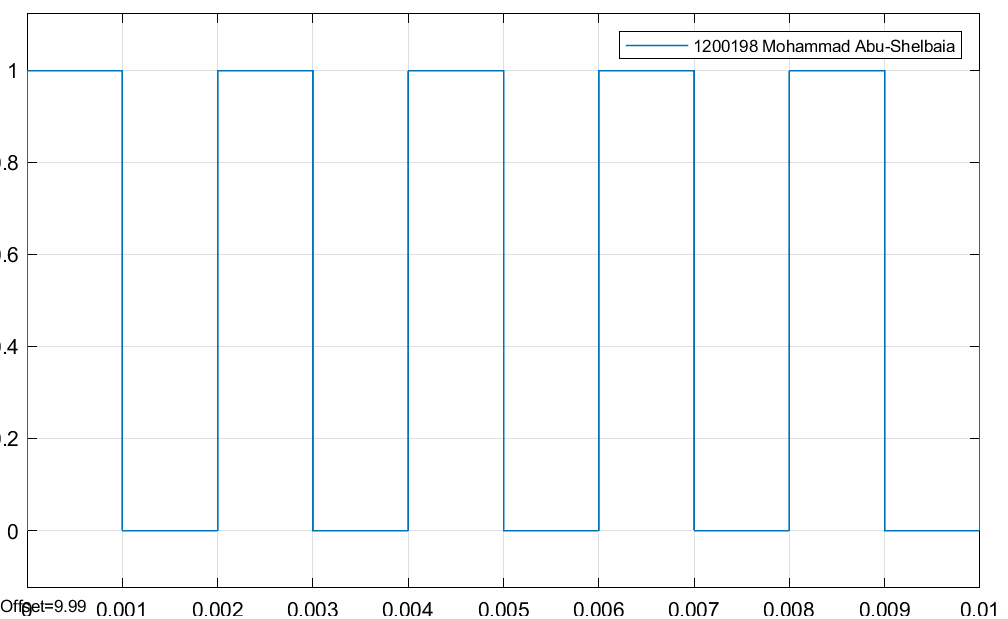
\includegraphics[width=\textwidth]{assets/main/2023-08-23-20-08-13.png}
    }
    \resizebox{0.49\textwidth}{0.25\textwidth}{
        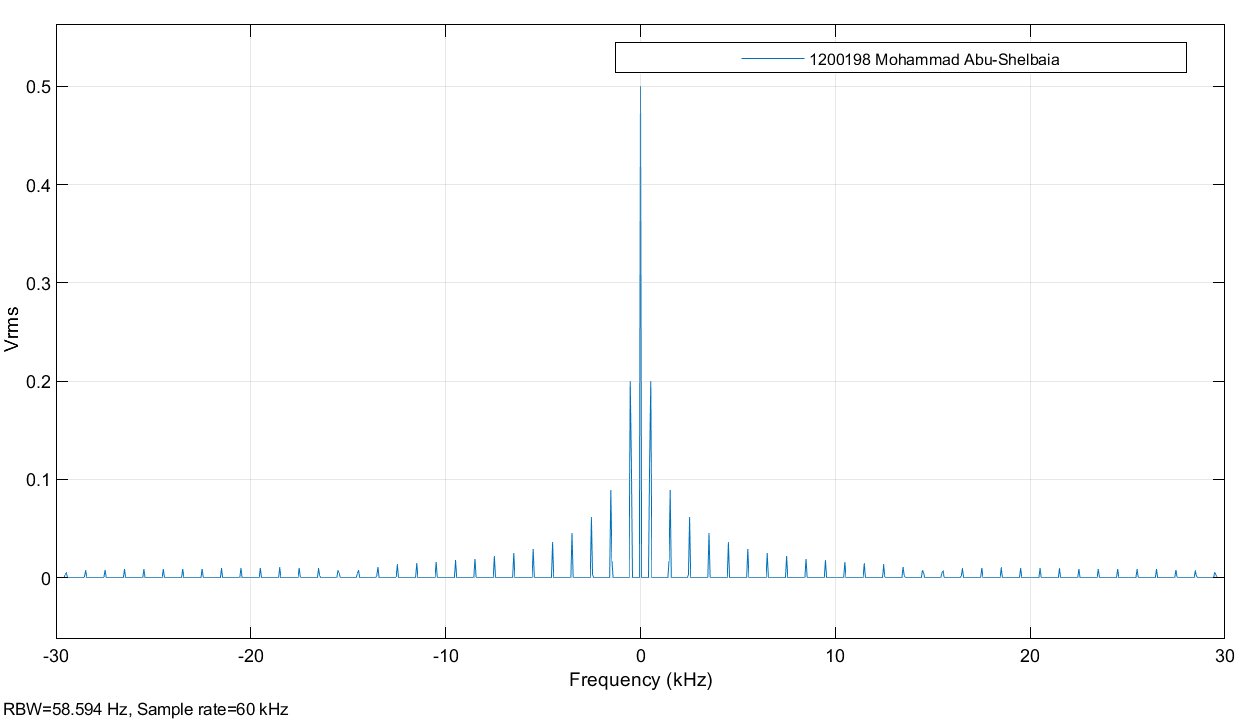
\includegraphics[width=\textwidth]{assets/main/2023-08-23-20-09-13.png}
    }
    \caption{Demodulated Singal Method 2 (500Hz)}
\end{figure}
We were able to recover the message signal dispite the low frequency.
\hhh{0.10 Duty-Cycle Modulating Signal}
\begin{figure}[H]
    \centering
    \resizebox{0.49\textwidth}{0.25\textwidth}{
    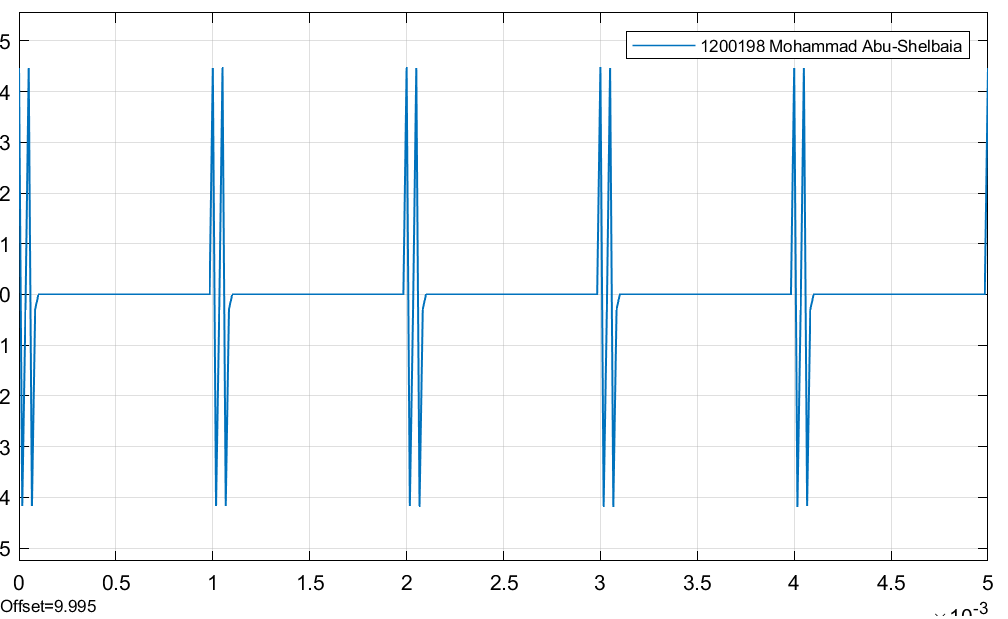
\includegraphics[width=\textwidth]{assets/main/2023-08-23-20-12-09.png}
    }
    \resizebox{0.49\textwidth}{0.25\textwidth}{
        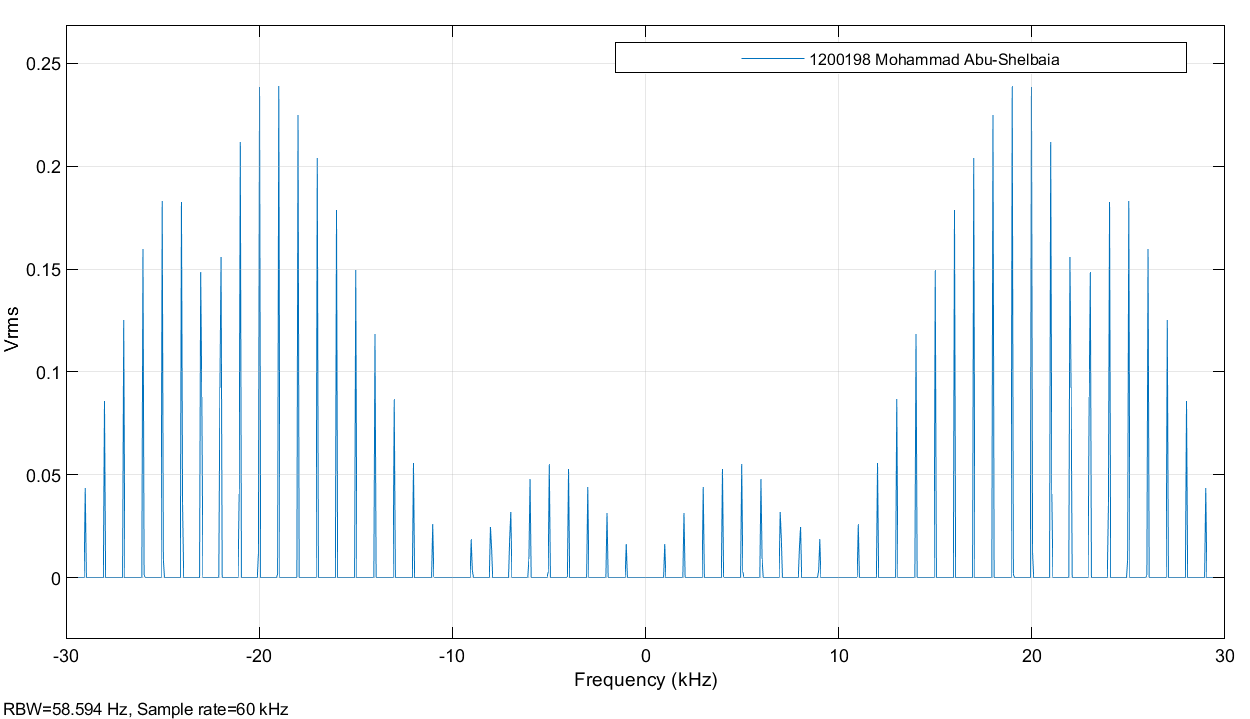
\includegraphics[width=\textwidth]{assets/main/2023-08-23-20-12-37.png}
    }
    \caption{Modulated Singal (10\% Duty Cycle)}
\end{figure}
We notice the the cosine repeated for only 2 times on the high portion of the message signal, and we further noticed that spectrum of the modulated signal is more dense with more frequencies.
\begin{figure}[H]
    \centering
    \resizebox{0.49\textwidth}{0.25\textwidth}{
    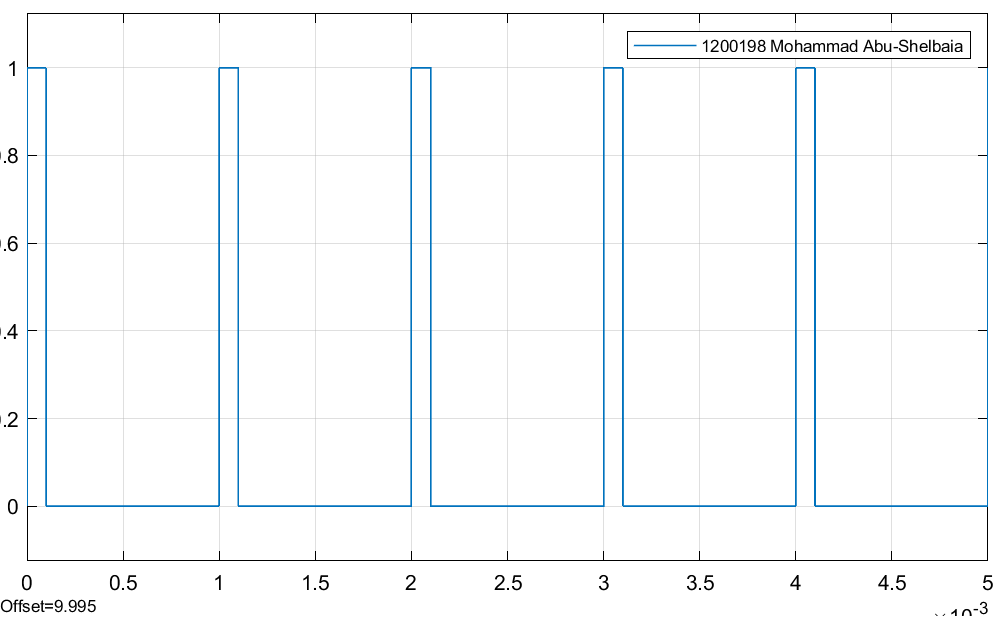
\includegraphics[width=\textwidth]{assets/main/2023-08-23-20-16-16.png}
    }
    \resizebox{0.49\textwidth}{0.25\textwidth}{
        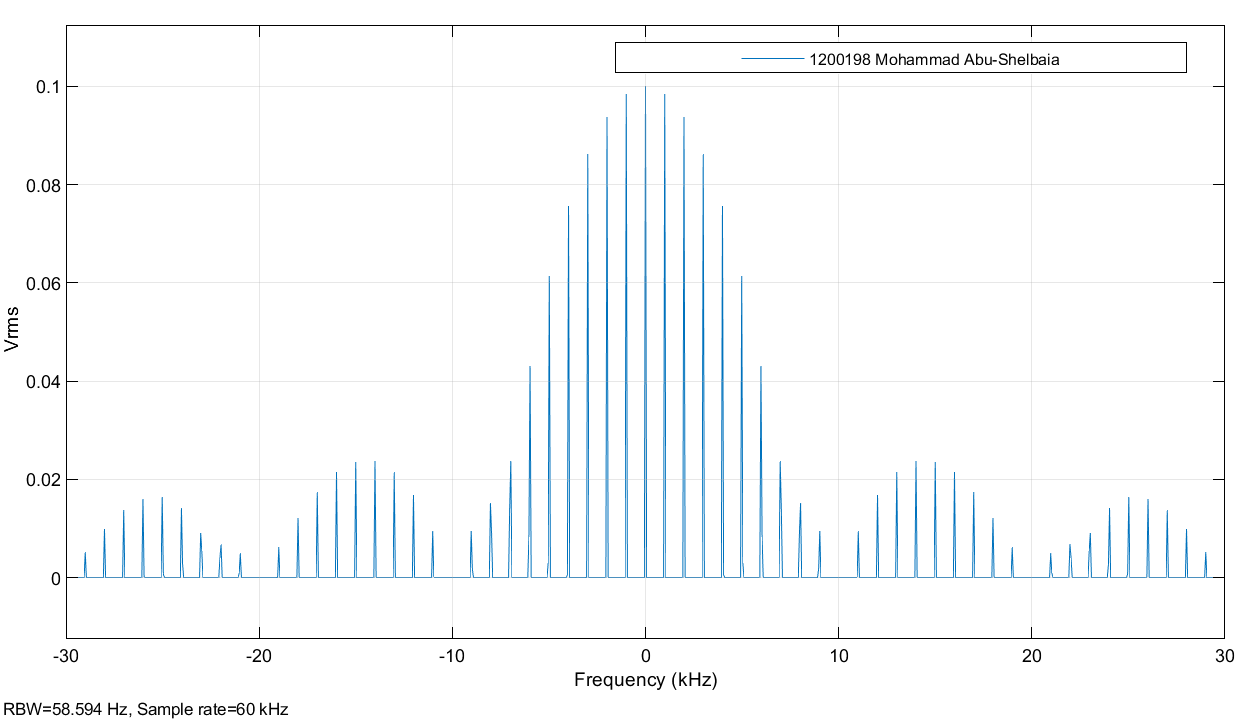
\includegraphics[width=\textwidth]{assets/main/2023-08-23-20-16-39.png}
    }
    \caption{Demodulated Singal Method 1  (10\% Duty Cycle)}
\end{figure}
\begin{figure}[H]
    \centering
    \resizebox{0.49\textwidth}{0.25\textwidth}{
    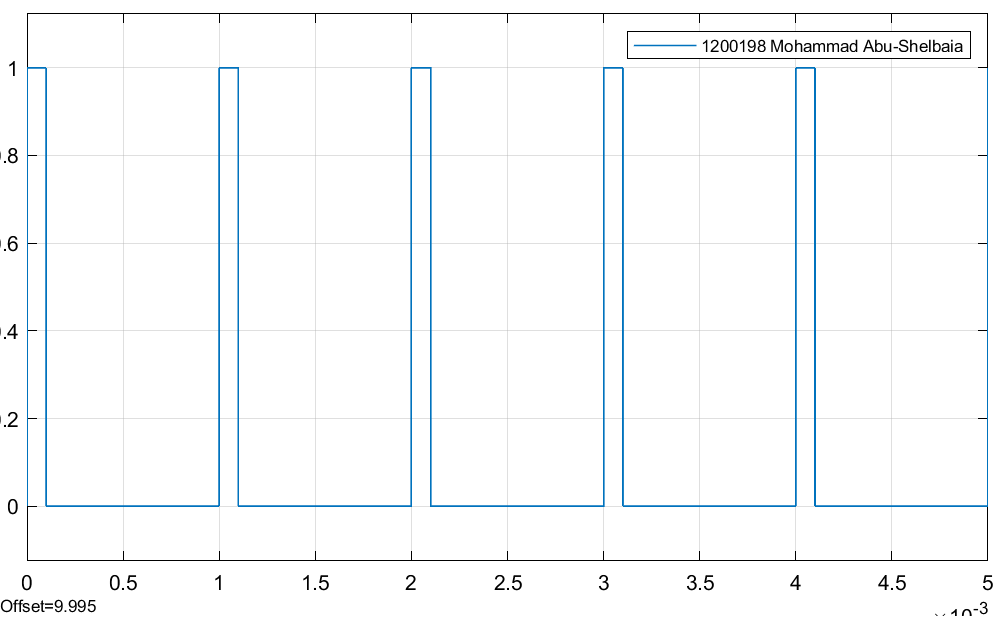
\includegraphics[width=\textwidth]{assets/main/2023-08-23-20-16-16.png}
    }
    \resizebox{0.49\textwidth}{0.25\textwidth}{
        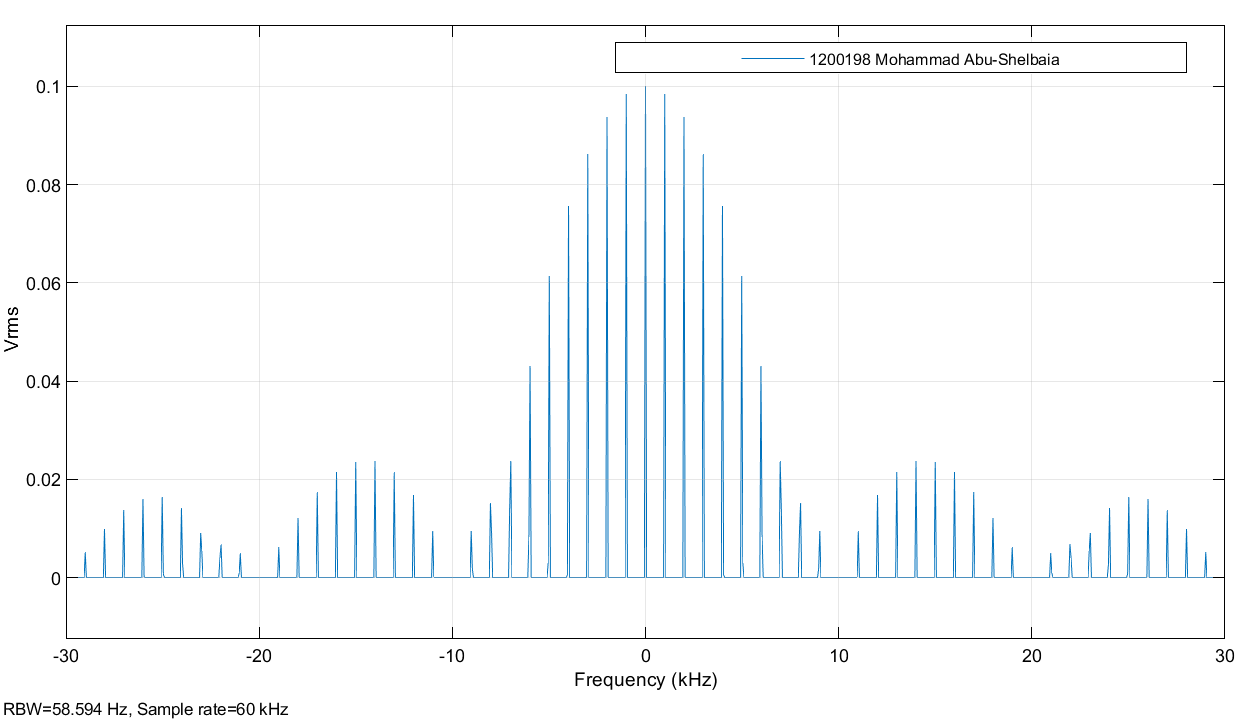
\includegraphics[width=\textwidth]{assets/main/2023-08-23-20-16-39.png}
    }
    \caption{Demodulated Singal Method 2  (10\% Duty Cycle)}
\end{figure}
We can see as all the previous parts we were able to recover the message correctly, the high portion of the message singal is recoverd as one, and the low portion is recovered as zero.
\end{document}





